%---------------------------------------------------------------------
%
%                         Project Name:Njust LabReport 
%
%---------------------------------------------------------------------
%
%                 created by Qingyun Fang <fqy2017@gmail.com>
%
%                        Last-modified: 2017-6-12
%
%---------------------------------------------------------------------

\documentclass[a4paper,12pt]{report}
\usepackage{ctex}
%\usepackage{xeCJK}
\usepackage{times}
\usepackage{setspace}
\usepackage{fancyhdr}
\usepackage{graphicx}
\usepackage{wrapfig}
\usepackage{array}  
\usepackage{fontspec,xunicode,xltxtra}
\usepackage{titlesec}
\usepackage{titletoc}
\usepackage[titletoc]{appendix}
\usepackage[top=30mm,bottom=30mm,left=20mm,right=20mm]{geometry}
\usepackage{cite}
\usepackage{listings}
\usepackage[framed,numbered,autolinebreaks,useliterate]{mcode} % 插入代码
\XeTeXlinebreaklocale "zh"
\XeTeXlinebreakskip = 0pt plus 1pt minus 0.1pt

%---------------------------------------------------------------------
%	页眉页脚设置
%---------------------------------------------------------------------
\fancypagestyle{plain}{
	\pagestyle{fancy}      %改变章节首页页眉
}

\pagestyle{fancy}
\lhead{\kaishu~通信工程实验报告~}
\rhead{\kaishu~913104330115~方青云~}
\cfoot{\thepage}

%---------------------------------------------------------------------
%	章节标题设置
%---------------------------------------------------------------------
\titleformat{\chapter}{\centering\zihao{-1}\heiti}{实验\chinese{chapter}}{1em}{}
\titlespacing{\chapter}{0pt}{*0}{*6}

%---------------------------------------------------------------------
%	摘要标题设置
%---------------------------------------------------------------------
\renewcommand{\abstractname}{\zihao{-3} 摘\quad 要}

%---------------------------------------------------------------------
%	参考文献设置
%---------------------------------------------------------------------
\renewcommand{\bibname}{\zihao{2}{\hspace{\fill}参\hspace{0.5em}考\hspace{0.5em}文\hspace{0.5em}献\hspace{\fill}}}

%---------------------------------------------------------------------
%	引用文献设置为上标
%---------------------------------------------------------------------
\makeatletter
\def\@cite#1#2{\textsuperscript{[{#1\if@tempswa , #2\fi}]}}
\makeatother

%---------------------------------------------------------------------
%	目录页设置
%---------------------------------------------------------------------
\titlecontents{chapter}[0em]{\songti\zihao{-4}}{\thecontentslabel\ }{}
{\hspace{.5em}\titlerule*[4pt]{$\cdot$}\contentspage}
\titlecontents{section}[2em]{\vspace{0.1\baselineskip}\songti\zihao{-4}}{\thecontentslabel\ }{}
{\hspace{.5em}\titlerule*[4pt]{$\cdot$}\contentspage}
\titlecontents{subsection}[4em]{\vspace{0.1\baselineskip}\songti\zihao{-4}}{\thecontentslabel\ }{}
{\hspace{.5em}\titlerule*[4pt]{$\cdot$}\contentspage}


\begin{document}
%---------------------------------------------------------------------
%	封面设置
%---------------------------------------------------------------------
\begin{titlepage}
	\begin{center}
		
    
\includegraphics[width=0.9\textwidth]{figure//Njust.png}\\
    \vspace{10mm}
    \textbf{\zihao{2}\kaishu{电子工程与光电技术学院}}\\[0.8cm]
    \textbf{\zihao{2}\kaishu{ 实验报告}}\\[3cm]
    
	\vspace{\fill}
	
\setlength{\extrarowheight}{3mm}
{\songti\zihao{3}	
\begin{tabular}{rl}
	
	{\makebox[4\ccwd][s]{班\qquad 级:}}& ~\kaishu 通信二班\\
	
	{\makebox[4\ccwd][s]{姓\qquad 名:}}& ~\kaishu 方青云 \\ 

    {\makebox[4\ccwd][s]{学\qquad 号:}}& ~\kaishu 913104330115 \\ 
   
	{\makebox[4\ccwd][s]{指导老师:}} & ~\kaishu 宁德强\\ 

\end{tabular}
 }\\[2cm]
\vspace{\fill}
\zihao{4}
2016\textasciitilde 2017第一学期\\
使用\LaTeX 撰写于\today
	\end{center}	
\end{titlepage}

%---------------------------------------------------------------------
%  摘要页
%---------------------------------------------------------------------
\begin{abstract}
\begin{spacing}{1.5}
	{\zihao{-4}
	南京理工大学(Nanjing University of Science and Technology)是中华人民共和国工业和信息化部直属的一所以工为主,理、工、文、经、管、法、教、艺等多学科协调发展的全国重点大学,是国家“211工程”、“985 工程优势学科创新平台”重点建设高校之一,是“111计划”、“卓越计划”、“中俄工科大学联盟”入选高校之一,素有“兵器技术人才摇篮”的美誉。
	
	1953年,南京理工大学由中国人民解放军军事工程学院(简称“哈军工”)分建而成,先后经历炮兵工程学院、华东工程学院、华东工学院等发展阶段,1993 年更为现名。
	
	学校北依紫金山,西临明城墙,校园占地3118亩。校舍建筑总面积98万平方米,
	南京理工大学是江苏唯一连续四届获得“江苏省十大专利金奖”和“十大专利发明人”称号的单位,并创办有全国第一个依托大学和大学科技园建设的国家专利产业化试点基地,为国防和国民经济建设均做出了重要贡献。\\[0.5cm]
	\textbf{关键字}:\quad 南理工 \quad 电光院 \quad 985平台 \quad211工程
	}
\end{spacing}
\end{abstract}

%---------------------------------------------------------------------
%  目录页
%---------------------------------------------------------------------
\tableofcontents % 生成目录

%---------------------------------------------------------------------
%  实验一
%---------------------------------------------------------------------
\chapter{电光13介绍}
\setcounter{page}{1}
\begin{spacing}{1.5}
\songti\zihao{-4}

\section{实验目的}
Happy TeXing!
\section{实验要求}
Happy TeXing!
\section{实验内容}
南京理工大学电子工程与光电技术学院2013级简称“电光13级”,是一个充满朝气,蓬勃向上的年轻集体\cite{Leslie.{1994}}。目前年级共有电子信息工程、通信工程、电子科学与技术、光电信息科学与工程、微电子技术、探测制导与控制技术、信息对抗技术7个专业,14个班级,563人,是全校2013级人数最多、规模最大的年级\cite{Donald.{1984}}。

\begin{figure}[htbp]
	\centering
	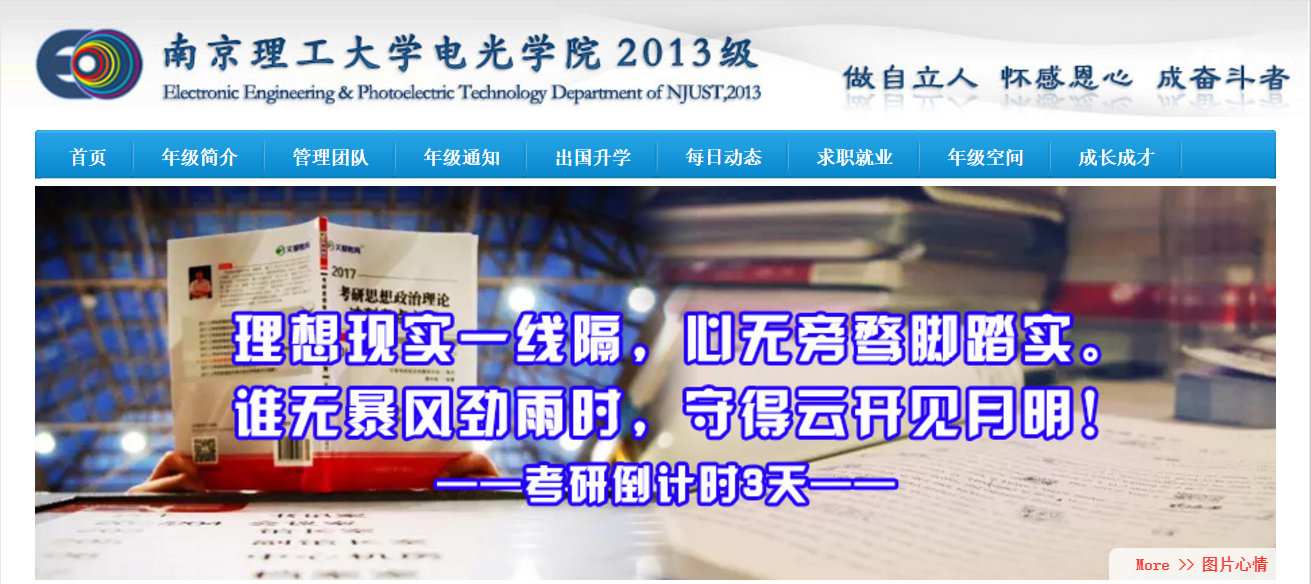
\includegraphics [width=1.0\textwidth]{figure//Fig1.png}
	\caption{南京理工电光13级}\label{dianguang13}
\end{figure}

电光13级拥有昂扬向上的年级文化。在学院层面年级秉承“敢为人先,争创一流”的电光精神,在年级层面提出打造“争先年级、团结年级、勤学年级、健康年级、追梦年级”的“五个年级”建设目标,在学生个人层面提出“做自立人,怀感恩心,成奋斗者”的培育目标,三个层面的文化理念共同构成年级的核心价值体系,成为激励电光13级广大同学奋斗进取的精神动力。同时,年级倡导“自立”文化、“感恩”文化和“奋斗”文化,注重将培养学生的热情意识、礼貌意识、时间意识和规则意识贯穿于育人工作始终。

电光13级拥有科学完善的年级制度。年级制定了包括《班级量化考核管理规定》、《学生综合素质测评规定》、《跑操考核规定》、《学生查课规定》、《卫生检查规定》、《宿舍检查规定》、《电脑使用管理规定》、《参与学术文化活动规定》、《请销假管理规定》、《住宿管理规定》等“十项规定”;划定了严禁“考试作弊、不假离校、擅自租房、私烧电器、滋事打架、私刻公章”的“六条红线”,形成了“十规六线”的制度系统。年级实现了制度规范的“上墙、上网、入脑、入心”,形成了人人遵守制度、人人敬畏制度、按制度行事的良好风气,保证了年级的“自动化管理”。年级正在积极起草《年级公约》,并将以公约为依据倡导广大同学实现自我教育、自我管理和自我服务。

电光13级拥有充满责任感的年级骨干。班长团支书队伍是各班的领跑者,按照“吃苦、吃亏、吃醋”的工作准则,在建设优秀班集体过程中发挥了核心作用。“三自”中心是年级学生自我教育、管理和服务的组织,承担日常“三查”和“三自论坛”工作。团学联合会是年级重要的群团组织,按照“团结型、奉献型、开放型”建设目标,负责各类文体和主题教育活动举办。党支部是学生党员组成的先锋组织,主要负责各类志愿服务活动开展。年级还设有秉承“精、专、敏、毅”工作准则的学习副班长工作组,秉承爱心、耐心、恒心“三心合一”理念的心理委员工作组等机构。年级骨干队伍的敬业、热情和无私奉献,是年级高效运行的坚实基础。

\begin{wrapfigure}{l}{0.33\textwidth}
	\begin{center}
		
\includegraphics[width=0.30\textwidth]{figure//Fig2.png}\\
	\end{center}
	\caption{EEschool}
\end{wrapfigure}

电光13级拥有争先进取的年级学风。年级借用“我为什么来到南理工?我想成为什么样的人?”的“竺可桢之问”,激励学生增强学习内驱力。实施严格的夜间查寝制、电脑承诺使用制、夜间集体自习制和“弹性化”的跑操制,并试行特等奖学金公开差额答辩制,多次举办“身边榜样故事”报告会等,通过班级和学生个人之间“比、学、赶、帮、超”的“标杆管理”模式,营造了年级内部时刻保持争先、向上、激活状态的浓郁学习氛围。年级学生英语四级通过率、计算机二级通过率、期末考试优秀率居于全校同年级前列。电光13级拥有丰富多元的年级活动。年级凡是有利于学生成长的活动都激励广大同学举办,凡是学校举办的重大集体活动都激励学生参加,凡是参加的活动都激励学生永争第一。年级先后积极参加了校院举办的新生运动会、新生舞龙大赛等活动,举办了年级“双旦”晚会、PPT大赛、寝室美化大赛、青春多米诺大赛、原创诗歌大赛等文体活动,并试行了年级兴趣活动的“大专业承办制”。各类活动中坚持事前有策划、事中有组织、事后有反思的“前中后三段论模式”,为丰富同学课余生活、提高同学综合素质,搭建了优良平台。

电光13级拥有高度敬业的管理团队。年级教育班是全年级整体教育、管理的负责机构,年级主任为宁德强,四名教育班学生助理为郭琪敏、郑星鑫、陈涵杰、陈璇。工作中,年级主任始终将“真爱学生”作为第一准则,秉承“用心、用脑、用感情”的育人理念,做广大学生的人生导师和知心朋友,工作中坚持不求成效的“立竿见影”,但求育人的“润物无声”。四位教育班助理秉承“甘当基石,愿为阶梯”的精神,协助辅导员做好年级工作。同时,教育班确定了工作中的“首问”负责制、“横向到边,纵向到底”分工制、“管理AB角”制、定期例会制等,保证了教育班和年级工作的正常、高效运转。

展望未来,电光13的优秀学子们将继续坚守“敢为人先,争创一流”的电光精神,倡导“自立、感恩、奋斗”的年级文化,以理想为帆,以行动为桨,为建设“争先、团结、勤学、健康、追梦”的电光13级而不断迈进、大步向前!

\section{实验分析}
Happy TeXing!
\end{spacing}

%---------------------------------------------------------------------
%  实验二
%---------------------------------------------------------------------
\chapter{通信二班}

\begin{spacing}{1.5}
\section{实验目的}

\section{实验要求}

\section{实验内容}

\section{实验分析}

\end{spacing}

%---------------------------------------------------------------------
%  实验感想
%---------------------------------------------------------------------
\titleformat{\chapter}{\centering\zihao{-1}\heiti}{}{1em}{}
\chapter{实验感想}
\begin{spacing}{1.5}
	没什么好说的。
\end{spacing}

%---------------------------------------------------------------------
%  参考文献设置
%---------------------------------------------------------------------
\addcontentsline{toc}{chapter}{参考文献}

\begin{thebibliography}{99}
\songti \zihao{-4} 	
	\bibitem{Leslie.{1994}}
	Leslie Lamport. LATEX: A Document Preparation System.AddisonWesley, Reading, Massachusetts, second edition, 1994, ISBN 0-201-52983-1.
	
	\bibitem{Donald.{1984}}
	Donald E. Knuth. The TEXbook, Volume A of Computers and Typesetting,Addison Wesley, Reading, Massachusetts, second edition, 1984,ISBN 0-201-13448-9.

	
\end{thebibliography}

%---------------------------------------------------------------------
%  附录设置
%---------------------------------------------------------------------
\titleformat{\chapter}{\heiti\Large}{附录~\Alph{chapter}}{11pt}{\Large}
\titlespacing{\chapter}{0pt}{*-4}{*4}

\lstset{breaklines}                %自动将长的代码行换行排版
\lstset{extendedchars=false}
\lstset{language=Matlab}
\renewcommand{\thechapter}{附录\Alph{chapter}.} 
\appendix
\begin{appendix}
	
	
\chapter{数据表}
\zihao{-4}\songti
\begin{spacing}{1.5}
	hello world!
\end{spacing}


\chapter{程序代码}
\zihao{-4}\songti
\begin{spacing}{1.5}
下面是一个MATLAB程序的事例,使用了Package mcode,它能较好还原MATLAB本身的编写风格。
\begin{lstlisting}
%The program normalizes the measurement data and compares it to the standard cosine function
data=xlsread('data_sun',1,'B3:E39');
min=[(data(1,1)+data(37,1))/2,(data(1,2)+data(37,2))/2,...
(data(1,3)+data(37,3))/2,(data(1,4)+data(37,4))/2];
max=[data(19,1),data(19,2),data(19,3),data(19,4)];
Min=repmat(min,37,1);
Max=repmat(max,37,1);
data=(data-Min)./(Max-Min);
x=-pi/2:pi/36:pi/2;
y=cos(x);
%----------------------figure-------------------------%
figure(1);
subplot(2,2,1);
plot(x,data(:,1),'ro-');
hold on;
plot(x,y,'b-');
title('R=1.2\Omega');
axis([-2,2,0,1]);
grid on;
subplot(2,2,2);
plot(x,data(:,2),'ro-');
hold on;
plot(x,y,'b-');
title('R=1.6\Omega');
axis([-2,2,0,1]);
grid on;
subplot(2,2,3);
plot(x,data(:,2),'ro-');
hold on;
plot(x,y,'b-');
title('R=2.0\Omega');
axis([-2,2,0,1]);
grid on;
subplot(2,2,4);
plot(x,data(:,4),'ro-');
hold on;
plot(x,y,'b-');
title('R=2.4\Omega');
grid on;
axis([-2,2,0,1]);
\end{lstlisting}
\end{spacing}
\end{appendix}
		

\end{document}